\section{Long-Term Temperature Trends in High Alpine Regions (RQ1)}

\subsection*{Objective}
This research question investigates whether long-term temperature trends differ by elevation. To illustrate the phenomenon of elevation-dependent warming, this section focuses specifically on the highest elevation category: \textbf{2000+\,m (High Alpine)}. These zones are climatically sensitive and relevant for alpine climate analysis.

\subsection*{Methodology}
Using Apache Spark, monthly average temperature values (\texttt{tl\_mittel}) from the full dataset \texttt{climate\_all\_stations} were grouped by station and year. Elevation metadata was joined and used to classify each station into one of five predefined elevation bands.

To ensure focus and clarity, this analysis considers only the High Alpine category. The reasoning is threefold:
\begin{itemize}
    \item It is directly linked to climate vulnerability and snow cover dynamics.
    \item It exhibits strong and distinctive warming signals.
    \item It includes representative stations from multiple federal states.
\end{itemize}

Two additional plots were generated for context:
\begin{itemize}
    \item A distribution plot of all stations by elevation zone and region.
    \item A labeled diagram of the highest station per region to confirm extreme values.
\end{itemize}

\subsection*{Results and Interpretation}

\paragraph{Figure~\ref{fig:temptrend_highalpine}: Temperature Trends in the High Alpine Zone}
The line plot below shows annual average temperatures from 1970 to 2025 for each region in the High Alpine zone. A general increase is evident. While Tyrol and Vorarlberg exhibit consistent warming, Salzburg remains colder on average. Differences could be due to regional geography or data coverage.

\begin{figure}[htbp]
    \centering
    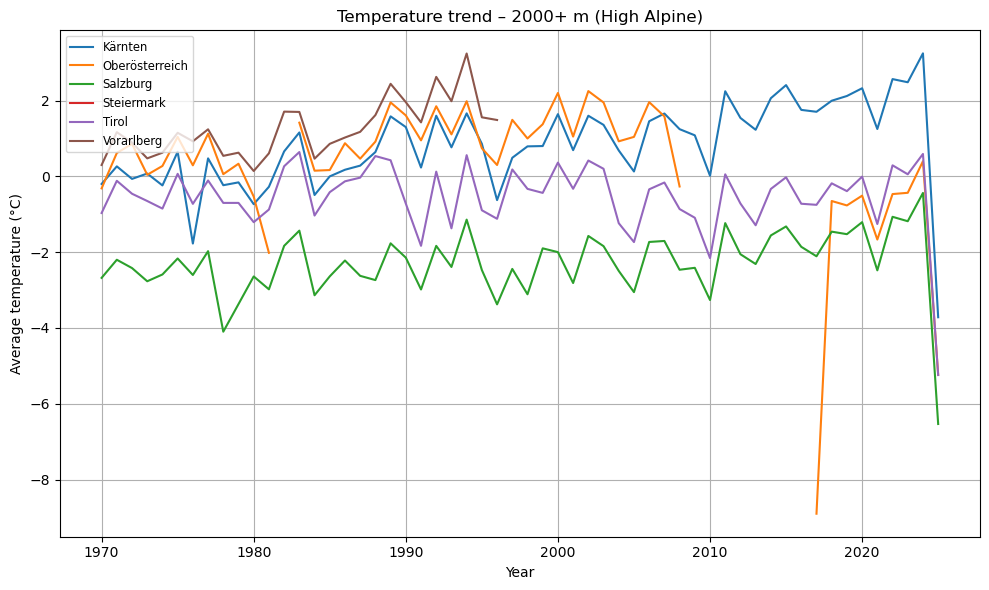
\includegraphics[width=\textwidth]{img/temptrend_highalpine.png}
    \caption{Average annual temperature trends (1970–2025) in 2000+\m High Alpine zone}
    \label{fig:temptrend_highalpine}
\end{figure}

\paragraph{Figure~\ref{fig:station_distribution_highalpine}: Altitude Distribution of High Alpine Stations}
This scatterplot validates that stations assigned to the High Alpine zone are located well above 2000+\m. The distribution also shows regional diversity, which supports cross-regional comparisons.

\begin{figure}[htbp]
    \centering
    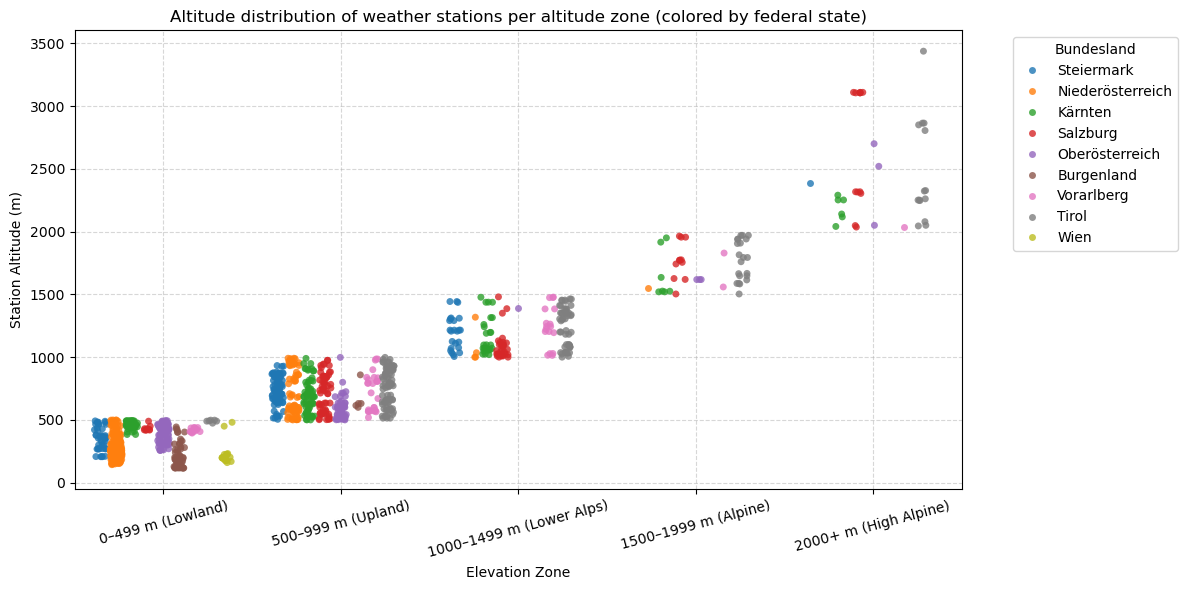
\includegraphics[width=\textwidth]{img/station_distribution_highalpine.png}
    \caption{Elevation distribution of stations by zone and region}
    \label{fig:station_distribution_highalpine}
\end{figure}

\paragraph{Figure~\ref{fig:highest_stations_labeled}: Highest Stations per Region}
This annotated plot confirms the locations and elevations of the highest weather stations per federal state. These are concentrated in Tyrol, Salzburg, and Carinthia—regions with substantial alpine terrain.

\begin{figure}[htbp]
    \centering
    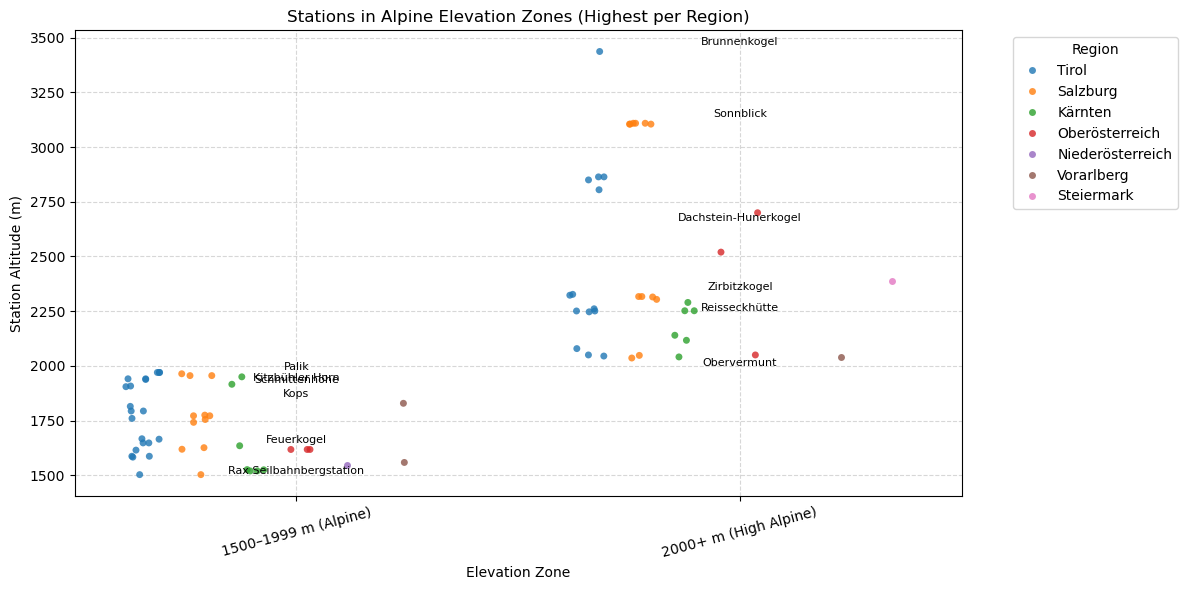
\includegraphics[width=\textwidth]{img/highest_stations_labeled.png}
    \caption{Highest station per region in Alpine zones with labels}
    \label{fig:highest_stations_labeled}
\end{figure}

\subsection*{Conclusion}
The High Alpine zone (2000+\m) in Austria shows a clear warming trend over the last five decades. Regional variation is present but does not detract from the overall pattern. By isolating a single elevation zone, this analysis enables focused insight while demonstrating elevation-dependent climate change.

The Spark-based implementation, which joins climate records with station metadata and performs grouped aggregations by year, proves efficient for scalable trend analysis. This framework can easily be extended to other elevation bands or regions.
